\section{Executed numerical experiments}\label{sec:experiments}

\subsection{Protocol}

\noindent All experiments were executed in Python~3.13 with NumPy~2.5 and SciPy~1.18 using fixed \texttt{SeedSequence} seeds
(Table~\ref{tab:experiments}). Parameter values are dimensionless illustrations, not estimates of ancestral heritability or
selection. Monte Carlo standard errors are between-replicate standard deviations divided by the square root of the number of
replicates; they measure computational precision only. Where a table reports the largest standardized deviation $|z|$ across
many comparisons, the number of comparisons is given, since a maximum near 2.5 is expected among twenty to forty independent
checks. The code was written from the equations in Section~\ref{sec:theory}; for the pair-output baseline at $n=32$, $\rho=0$,
for example, the exact response is \EOneExact{} and the Monte Carlo mean \EOneMC.

\begin{table*}[t]
\caption{Executed experiments and verification outcomes.}\label{tab:experiments}
\scriptsize
\begin{tabularx}{\textwidth}{@{}P{0.035\textwidth}P{0.14\textwidth}P{0.33\textwidth}Lr@{}}
\toprule
ID & Purpose & Design & Verification outcome & Seed\\
\midrule
E1 & Pair-output baseline & 20 replicates $\times$ 20,000 pairs; 18 repetition conditions plus random pairing &
Max $|\text{MC}-\text{exact}|=\EOneMaxDiff$ & 20261109\\
E2 & Proposition~\ref{prop:routes} & 3 scenarios $\times$ 7 validity values; 20 replicates $\times$ 20,000 per sex &
Max $|z|=\ETwoMaxZ$ over \ETwoN{} comparisons & 20261111\\
E3 & Propositions~\ref{prop:portfolio}--\ref{prop:diversity} & 8 splits of a 24-event budget (20 replicates $\times10^5$) plus
repeat-versus-diverse series & Max $|z|=\EThreeMaxZ$ over \EThreeN{} comparisons & 20261112\\
E4 & Proposition~\ref{prop:assort} & Individual-based; 5,000 per sex; 150 generations; 10 replicates; 5 conditions &
Final means and $V_A$ within \MGerr\% of the recursion & 20261113\\
E5 & Decentralized matching, non-display & Men-proposing deferred acceptance, 1,000 per sex, 15 replicates; non-display
with $2\times10^5$ individuals & Response within $\DAdiff$ of $bV_A(1+m)/2$ & 20261114\\
E6 & Propositions~\ref{prop:persist}--\ref{prop:tissue} & Individual-based equilibrium (5,000 per sex, 1,500 generations, 6
replicates); deterministic bivariate dynamics & Equilibrium $\PersSim\pm\PersSD$ (SD) against predicted \PersPred & 20261115\\
E7 & Rate audit, envelope & Analytic grids from published summaries & Tables~\ref{tab:rates},~\ref{tab:drift},~\ref{tab:envelope} &
---\\
E8 & Stage-2 power & Crossed observer $\times$ target simulation, 500 replicates per cell & Fig.~\ref{fig:power} & 20261116\\
E9 & Proposition~\ref{prop:identity} & 4 allocation shapes $\times$ 5 validities, $2\times10^5$ individuals, 20 replicates;
Laplace traits; pair-output model at fixed opportunity & Max $|z|=\ENineMaxZ$ over \ENineN; bound never violated & 20261118\\
E10 & Proposition~\ref{prop:aim}, Corollary~\ref{cor:cue} & 3 regimes $\times$ 2 allocation rules, $2\times10^5$ individuals, 20
replicates; state-dominated cue & Max $|z|=\AimMaxZ$ over \AimN{} comparisons & 20261120\\
E11 & Proposition~\ref{prop:repeat} & Validity for 1--64 explicit events ($10^5$ individuals, 20 replicates); optimum by
root-finding and by grid search & Max $|z|=\RepMaxZ$; $n^*$ monotone in $\delta/B$ & 20261121\\
E12 & Proposition~\ref{prop:despot} & Grid over rival strength, share and contest exponent; first-order root against
brute-force maximum & Log-concavity, monotonicity and limit confirmed & ---\\
E13 & Fossil reanalysis & Three open datasets; model comparison; \FosBoot{} bootstrap resamples & Section~\ref{sec:explananda};
Fig.~\ref{fig:fossils} & 20261119\\
E14 & Present-day decomposition (Proposition~\ref{prop:episodes}) & General Social Survey 1972--2024, \GssN{} respondents aged
45--79; \GssBoot{} bootstrap resamples; five robustness variants; three-episode and fifths analyses & Access and number sum to
the total to $\le\GssCheck$; Tables~\ref{tab:gss},~\ref{tab:gsscohort}--\ref{tab:gssthree} & 20261110\\
E15 & Propositions~\ref{prop:time}--\ref{prop:division}, Corollary~\ref{cor:generalist} & Aim ratio for 1--16 common domains and
1--20 specialties ($3$--$4\times10^5$ individuals, 20 replicates); individual-based evolution of general and specific
investment (20,000 individuals, 700 generations, 15 conditions $\times$ 4 replicates) & Aim ratio within \PolyAimErr\% of
$K V_{A,G}/V_{A,S}$; expenditure share within \PolyShareErr{} of Eq.~\eqref{eq:share}; Figs.~\ref{fig:main}C,~\ref{fig:polymath} & 20261121\\
E16 & Propositions~\ref{prop:staging}--\ref{prop:enforce} & Validity for capacity and delivery at seven staging shares
($3\times10^5$ candidates, 20 replicates); equilibrium under enforcement by closed form, by iteration and by
individual-based evolution (20,000 individuals, 2,000 generations, 6 levels $\times$ 3 replicates) & Validities within
\VerMaxDiff{} of Eq.~\eqref{eq:staging}; equilibria within \EnfIbmDiff{} of Eq.~\eqref{eq:enforceeq};
Figs.~\ref{fig:main}D,~\ref{fig:verify} & 20261123\\
E17 & Agreement among observers; said and did (Section~\ref{sec:speed}) & Columbia speed-dating file, \SdRows{} meetings of
\SdN{} people; split-panel agreement for panels of 1--8 (400 draws); linear probability models with chooser fixed effects;
bootstraps over persons & Agreement within \JurGapMax{} of Eq.~\eqref{eq:sb}; Figs.~\ref{fig:main}B,~\ref{fig:jury};
Table~\ref{tab:speed} & 20261124\\
E18 & Who decides, constraint and coercion (Section~\ref{sec:reschoice}) & D-PLACE release of the Standard Cross-Cultural
Sample, Ethnographic Atlas and Binford's compilation; tabulation of published codes; bootstraps over groups for the forager
age gap & Table~\ref{tab:cultures}; Fig.~\ref{fig:choice}A--C & 20261126\\
E19 & Ancestors, births, ideals, ties (Sections~\ref{sec:ressexes},~\ref{sec:resvillage}) & General Social Survey, second
extract; effective numbers on completed families; decomposition of a difference between two rates; linear probability
model; 300--500 bootstraps & Tables~\ref{tab:births},~\ref{tab:village}; Figs.~\ref{fig:main}F,~\ref{fig:choice}D,~\ref{fig:village} & 20261127\\
E20 & Ideals and pairing across countries (Section~\ref{sec:resculture}) & 175-country file (\WdN{} rows) and 45-country
file (\WtN{} rows); country-level differences; fixed-effects linear probability model; 1{,}000 resamples of countries &
Table~\ref{tab:world}; Fig.~\ref{fig:world} & 20261128\\
E21 & Proposition~\ref{prop:ancestors},~\ref{prop:waiting}; Corollaries~\ref{cor:ritual},~\ref{cor:narrow};
Eq.~\eqref{eq:coercion} & Drift at a uniparental marker with 4{,}000 parents and 6{,}000 replicates per cell; simulated
panels, trials, domains and mixtures & Effective number within \NtAncErr\%; other checks within \NtWaitErr{} to
\NtNarErr & 20261129\\
A1--A17 & Independent audit & Conditional-Gaussian construction; quadrature; root versus iteration; covariance algebra;
direct maximization; exact summation; recomputation from raw files; exact enumeration; recounts by a second reader & Max $|z|=\AudZ$; exact checks agree to $\le\AudEq$ (Section~\ref{sec:auditnum}) & 20261117\\
\bottomrule
\end{tabularx}
\end{table*}

\subsection{The information--opportunity identity}

Experiment~E9 tests Proposition~\ref{prop:identity} with four allocation rules that differ greatly in shape: exponential
allocation (the standing route), a bounded percentile-acceptance rule, truncation at the median, and a convex rule that
quadruples the contribution of roughly the top sixth. For each rule the opportunity $\CV(W)$ is the same at every validity,
and the response divided by $\sqrt{R}$ is constant to within Monte Carlo error (Table~\ref{tab:identity}). The percentile
rule attains \PctEff\% of the Cauchy--Schwarz bound. With heavy-tailed (Laplace) breeding values, environments, and errors,
the linear prediction errs by up to \LapWorst\% (truncation at $R=\LapWorstR$), but the bound computed from a binned
conditional expectation is never violated. Finally, holding the variance of log pair output fixed in the pair-output model,
the response rises from \FixLo{} to \FixHi{} as $R$ goes from 0 to 1, a factor of \FixRatio, that is $\sqrt2$, rather than 2.

\begin{table}[t]
\caption{Information at fixed opportunity (E9): response divided by $\sqrt R$.}\label{tab:identity}
\footnotesize
\begin{tabularx}{\columnwidth}{@{}Xcccc@{}}
\toprule
Allocation rule & $\CV(W)$ & $R=0.1$ & $R=0.5$ & $R=1$\\
\midrule
\tabinput{generated/tab_identity.tex}
\bottomrule
\end{tabularx}
\tablenote{$V_A=0.4$, $V_P=1$. Pair-output model with $\Var(\ln W)$ held fixed: response \FixLo{} at $R=0$ and \FixHi{} at
$R=1$.}
\end{table}

\subsection{Three routes and portfolios}

Fig.~\ref{fig:routes}A confirms Proposition~\ref{prop:routes} for three scenarios: a pair-output model, the same
model with a standing effect, and status-dependent mating success in men without any assortment. Adding a modest standing
coefficient ($\beta_S=0.1$) raises the response at $R=1$ from $2.0\times$ to $3.0\times$ the information-free baseline within a
single generation. Part of that gain comes from assortment raising the inequality of pair output; the standing component is a
pure information effect. The concave $\sqrt R$ shape means much of the standing benefit is available at moderate validity.

Fig.~\ref{fig:routes}B confirms Proposition~\ref{prop:portfolio}. With 64 observed events, putting every event in a new
domain gives $R_G=\PortDiv$, against \PortRep{} for 64 repetitions in one domain, which cannot exceed its ceiling of
\PortCeilS. For a fixed budget of 24 events, moving from 1 to 24 domains raises the selection differential on general
capacity by a factor of \PortSGratio{} (from \PortSGa{} to \PortSGb) and lowers the push on each specialized skill
\PortSSratio-fold (from \PortSSa{} to \PortSSb).

\begin{figure*}[t]
\centering
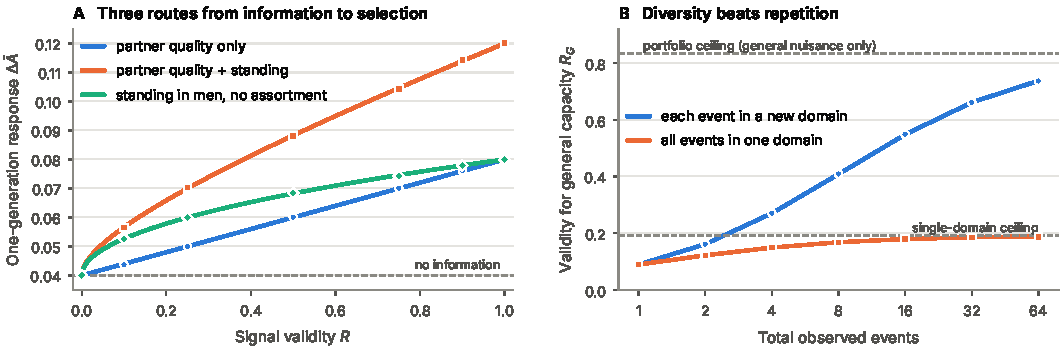
\includegraphics[width=\textwidth]{figures/figS1_routes.pdf}
\caption{\textbf{Routes and portfolios.} \textbf{(A)}~One-generation response under three routes ($V_A=0.4$, $V_P=1$): a
pair-output model ($b=0.2$); the same plus standing ($\beta_S=0.1$); and standing-dependent mating success in men
only ($\beta_N=0.1$, $\beta_S=0.2$), with no assortment. Lines: Eq.~\eqref{eq:threeroute}; markers: Monte Carlo means $\pm2$
standard errors (E2). \textbf{(B)}~Validity for general capacity when a fixed number of events is spread across new domains
or repeated within one; dashed lines are the ceilings of Proposition~\ref{prop:portfolio}. Parameters: $V_G=V_S=0.5$,
$\tau^2=0.5$, $\sigma^2=4$, $\rho=0.25$, $\omega^2=0.1$ (E3). Synthetic calculations, not estimates of human parameters.}
\label{fig:routes}
\end{figure*}

\subsection{Multigenerational amplification}

Fig.~\ref{fig:multigen} shows the individual-based simulation of Proposition~\ref{prop:assort}. With pair output $b=0.05$
and genic heritability 0.4, rank matching on observed scores raised additive variance to \MGva{} for initial validities
0.40, 0.67, 0.91, and 1, matching the recursion to within \MGerr\%. After 150 generations the cumulative response relative
to random pairing was \MGratio; the corresponding equilibrium amplifications are \MGF. The single-generation ceiling of two is
therefore not a ceiling on evolution. These ratios hold the pair-output coefficient fixed and so include the opportunity
increase that assortment creates. The genetic part is unambiguous: additive variance itself rose \MGinflLo- to
\MGinflHi-fold.

\begin{figure*}[t]
\centering
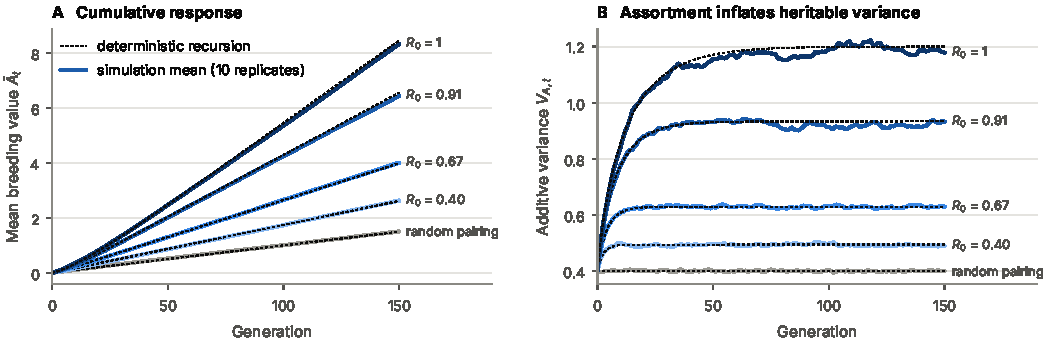
\includegraphics[width=\textwidth]{figures/figS2_multigen.pdf}
\caption{\textbf{Assortment across generations} (E4). Individual-based infinitesimal-model simulation: 5,000 individuals per
sex, 10 replicates, pair output $b=0.05$, $V_{LE}=0.4$, $V_E=0.6$. Partners are rank-matched on scores with fixed observation
noise; $R_0$ is the initial validity. Solid: simulation means; dotted: Eq.~\eqref{eq:assort} with mean response
$\tfrac b2V_{A,t}(1+m_t)$. Synthetic calculations.}
\label{fig:multigen}
\end{figure*}

\subsection{Decentralized matching and strategic non-display}

Ideal rank matching is a strong assumption. Experiment~E5 replaces it with men-proposing deferred
acceptance~\cite{gale1962} in which each person ranks potential partners by standardized score plus an idiosyncratic taste
term with standard deviation $s$. With common rankings ($s=0$) the stable matching gives $m=\DAmZero$ at $R=0.5$.
Idiosyncratic taste lowers the partner correlation, to \DAmOne{} at $s=1$ and \DAmTwo{} at $s=2$ (Table~\ref{tab:robust}), but
the response continues to follow $bV_A(1+m)/2$. The partner-quality route is thus governed by the realized phenotypic partner
correlation, a quantity measurable in any population. Non-display was modeled in two ways. When a random fraction $q$ do not
perform, validity falls to $(1-q)R$. When the lowest-scoring fraction hides and observers infer that hiders are below
average, validity falls much less (\HideThr{} instead of \HideRand{} at $q=0.4$), as disclosure unraveling
predicts~\cite{milgrom1981}.

\begin{table}[t]
\caption{Robustness to decentralized matching and non-display ($R=0.5$; E5).}\label{tab:robust}
\footnotesize
\begin{tabularx}{\columnwidth}{@{}Xccc@{}}
\toprule
\tabinput{generated/tab_robust.tex}
\bottomrule
\end{tabularx}
\end{table}

\subsection{Persistence, budget, and tissue}

Fig.~\ref{fig:persist}B verifies Proposition~\ref{prop:persist} in a finite population whose variance, validity, and
heritability evolve freely under the cost: the simulated equilibrium was \PersSim{} (between-replicate SD~\PersSD) against
\PersPred{} predicted from the realized $R$ and $V_P$. Fig.~\ref{fig:persist}A iterates Proposition~\ref{prop:tissue} with
$a=0.5$, $\kappa_K=0.01$, $\beta_{\mathrm{eff}}=0.04$, and tissue cost $\kappa_B$ halved three times. Both benefit types
begin with the same marginal value. Under positional demand, tissue investment doubles with each halving (\TisPos~SD), as
Eq.~\eqref{eq:tissue} predicts. Under saturating ecological demand, the same budget relaxations yield \TisEco~SD. When
positional returns are halved in the final phase (decoupling), tissue falls back to \TisBack~SD; the ecological trajectory is
unaffected. The time constant of each step is \TisApproachLo{} to \TisApproachHi{} generations, so at fossil resolution the
trajectory reads as stasis and steps.

\begin{figure*}[t]
\centering
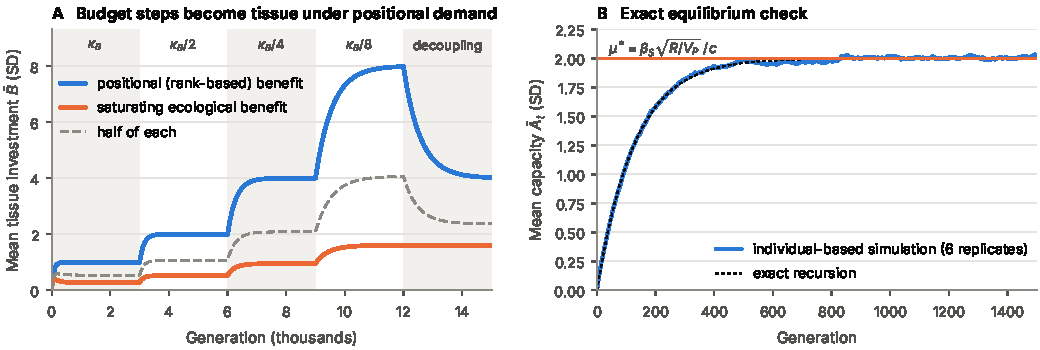
\includegraphics[width=\textwidth]{figures/figS3_persist.pdf}
\caption{\textbf{Persistence, budget, and tissue} (E6). \textbf{(A)}~Deterministic bivariate dynamics of
Proposition~\ref{prop:tissue}: tissue $B$ and organization $K$ with $\mathbf G=\mathrm{diag}(0.7,0.4)$, $a=0.5$,
$\kappa_K=0.01$, initial marginal benefit 0.04. Tissue cost $\kappa_B=0.02$ is halved at 3,000-generation intervals; in the
last phase positional returns are halved. \textbf{(B)}~Individual-based check of Proposition~\ref{prop:persist} (5,000 per
sex, 6 replicates, $c=0.02$, initial $R=0.5$); the horizontal line is Eq.~\eqref{eq:mustar} at realized $R$ and $V_P$.
Synthetic calculations, not fits to fossil data.}
\label{fig:persist}
\end{figure*}

\subsection{Contest, coalition, and aim}

Experiments E10--E12 check Model~V (Fig.~\ref{fig:contest}; Table~\ref{tab:modelv}). \emph{Aim.} Three illustrative regimes
weight three venues differently: a contest of force (loadings 1.0 on formidability and 0.25 on capacity), hunting (0.6 and
0.6), and verbal performance (0 and 1.0). With equal heritabilities, the simulated differentials match
Eq.~\eqref{eq:aim} under both an exponential rule ($\beta_S=0.2$) and a top-decile rule, and the ratio $S_{A_G}/S_{A_F}$ is
the same under both, as the proposition requires. Moving from the contest regime to skill and prestige raises selection on
capacity from \AimDomG{} to \AimPreG~SD and lowers selection on formidability from \AimDomF{} to \AimPreF. A cue in which 80\%
of the variance is a transient state yields a heritable response of only \CueSQ{} and no response in capacity
($|S_{A_G}|=\CueSG$, within one standard error of zero).

\emph{Repeatability.} With event noise four times the phenotypic variance, a single decisive contest has validity
\RepROne, against a ceiling of \RepCeil. As the cost per event falls from $\delta/B=0.2$ to $0.001$, the optimal number of
events rises from one to \RepNsafe{} and validity at the optimum to \RepRsafe, \RepFrac\% of the ceiling; at fixed intensity
the response is \RepGain{} times that of the single fight.

\emph{Leveling.} With subordinates' price $q=0.05$, a dominant tolerates no rivals until rival strength exceeds
$M=\DesThrLin$ fighter-equivalents under the linear law, or \DesThrSq{} under the square law. As $M$ grows his optimal share
falls toward \DesShareLin{} and \DesShareSq{} respectively, and the opportunity for selection among twenty males falls from
\DesIdespot{} to \DesILin{} and \DesISq.

\begin{figure*}[t]
\centering
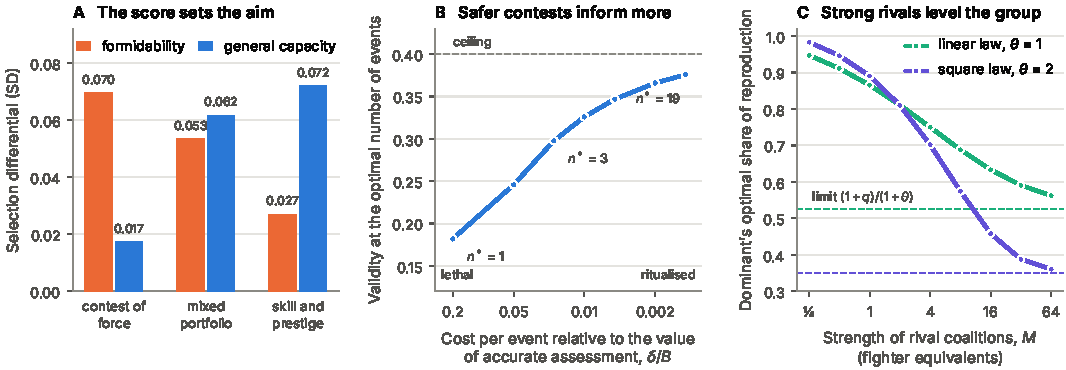
\includegraphics[width=\textwidth]{figures/figS4_contest.pdf}
\caption{\textbf{Contest, coalition, and aim} (E10--E12). \textbf{(A)}~Selection differentials on breeding values for
formidability and general capacity under three weightings of venues, at equal intensity (Proposition~\ref{prop:aim}).
\textbf{(B)}~Validity at the optimal number of contest events as the cost per event falls (Proposition~\ref{prop:repeat});
labels give $n^*$. \textbf{(C)}~The dominant's optimal share of reproduction as rival coalitions strengthen, with $q=0.05$
(Proposition~\ref{prop:despot}); dashed lines are the limits $(1+q)/(1+\theta)$. Loadings, costs and shares are
illustrative assumptions.}
\label{fig:contest}
\end{figure*}

\begin{table}[t]
\caption{Model~V illustrations (E10, E12). Loadings and shares are assumptions.}\label{tab:modelv}
\footnotesize
\begin{tabularx}{\columnwidth}{@{}Xccccc@{}}
\toprule
\multicolumn{6}{@{}l}{\textit{(a) Aim at equal intensity ($\beta_S=0.2$, $h^2=0.5$)}}\\
Regime & $\bar\ell_F$ & $\bar\ell_G$ & $S_{A_F}$ & $S_{A_G}$ & Ratio\\
\midrule
\tabinput{generated/tab_aim.tex}
\bottomrule
\end{tabularx}

\vspace{4pt}
\begin{tabularx}{\columnwidth}{@{}Xcccccc@{}}
\toprule
\multicolumn{7}{@{}l}{\textit{(b) The despot's dilemma ($q=0.05$; pool of 20 males)}}\\
 & \multicolumn{3}{c}{Linear law, $\theta=1$} & \multicolumn{3}{c}{Square law, $\theta=2$}\\
\cmidrule(lr){2-4}\cmidrule(l){5-7}
Rivals $M$ & $k^*$ & Share & $I$ & $k^*$ & Share & $I$\\
\midrule
\tabinput{generated/tab_despot.tex}
\bottomrule
\end{tabularx}
\tablenote{$k^*$: tolerated subordinates (integer optimum); Share: the dominant's share of group reproduction; $I$: opportunity
for selection among the 20 males, which is 19 when one male monopolizes reproduction.}
\end{table}

\subsection{The generalist target}

Experiment~E15 checks the results of Section~\ref{sec:generalist} (Figs.~\ref{fig:main}C and~\ref{fig:polymath}). With everyone compared on $K$
common domains, the simulated ratio of the selection differential on general capacity to that on one specialty is
\PolyRatioOne, \PolyRatioFour{} and \PolyRatioSixteen{} for $K=1$, 4 and 16, against exact values of 1, 4 and 16, while validity
for general capacity rises from \PolyValOne{} to \PolyValSixteen. When each individual is instead assessed only in the domain
of their greatest specific talent, the ratio is \PolyDivSimTen{} for ten specialties (exact, to first order in the strength of
selection, \PolyDivExTen), so common comparison aims \PolyDivTen{} times more strongly at general capacity than division of
labor does. Under a rule that honors each person's best performance while everyone is still seen in every domain, the
covariances are $V_G$ and $V_S/K$ as Stein's lemma requires, and only validity falls (from \PolySteinMean{} to \PolySteinMax{} at
$K=10$). In the individual-based evolution of a general investment and $K$ specific ones, the share of cost devoted to
general capacity matches Eq.~\eqref{eq:share} to within \PolyShareErr{} in all fifteen conditions, passing one half where the
number of domains equals the cost ratio.

\subsection{Tests and enforcement}

Experiment~E16 checks Section~\ref{sec:verification} (Figs.~\ref{fig:main}D and~\ref{fig:verify}A,B). Candidates were given a capacity, a default
rate drawn from a beta distribution with mean one quarter, and \VerN{} observed occasions split between staged and unstaged.
Simulated validities for capacity and for delivery agree with Eq.~\eqref{eq:staging} to within \VerMaxDiff{} at all seven
staging shares; the share that maximizes their product is \VerDstar, as Eq.~\eqref{eq:dstar} gives. For enforcement,
iterating the recursion for the means reproduces Eq.~\eqref{eq:enforceeq} to $\EnfRecErr$ both below and above the
threshold, and an individual-based population in which assessors shrink noisy signals of each trait settles within
\EnfIbmDiff{} of the predicted capacity and commitment at six levels of enforcement. With no enforcement and $T=\EnfT$
neither trait leaves zero; with complete enforcement capacity reaches its maximum and commitment stays at zero.

\subsection{Independent audit}\label{sec:auditnum}

A separate script re-derives each proposition by a different construction and imports no model code.
Proposition~\ref{prop:routes} was checked by constructing matched pairs directly from the conditional Gaussian distribution of
capacity given a shared score, with no sorting (40 blocks of 200,000 pairs; maximum $|z|=\AudZ$ across five validities);
Proposition~\ref{prop:persist} by 120-point Gauss--Hermite quadrature of the tilted density (maximum error $\AudQuad$);
Proposition~\ref{prop:assort} by comparing the quadratic root with fixed-point iteration (error $\AudRoot$, and divergence
confirmed where no equilibrium exists); Propositions~\ref{prop:portfolio} and~\ref{prop:aim} by explicit covariance algebra on
loading matrices (error $\AudCov$); Propositions~\ref{prop:repeat} and~\ref{prop:despot} by direct numerical maximization over
200 random parameter draws each (first-order residual $\AudFOC$; monotonicity confirmed; limiting share within $\AudAsym$);
and Proposition~\ref{prop:tissue} by iterating the dynamics for 20 random positive-definite $\mathbf G$ (equilibrium error
$\AudEq$, with tissue returning to zero when $a=0$). Corollary~\ref{cor:generalist} was checked by covariance algebra on
the loading vector and Proposition~\ref{prop:polymath} by iterating the dynamics for 20 random genetic covariance matrices
(error $\AudPoly$); the constants $c_K$ of Proposition~\ref{prop:division} by Monte Carlo (error $\AudCK$); and the
present-day decomposition by an independent implementation that reproduces every component of Table~\ref{tab:gss} checked to
$\AudGss$. Proposition~\ref{prop:delivery} was checked by Monte Carlo with $2\times10^6$ individuals (largest standardized
deviation \AudDelZ) and its threshold by the eigenvalues of 200 random systems, with no mismatch.
Proposition~\ref{prop:staging} was checked by exact summation over the default rate and the binomial count (error
$\AudStage$) and its optimum by bounded minimization (error $\AudStageOpt$); Proposition~\ref{prop:enforce} by Monte Carlo
covariances (largest standardized deviation \AudEnfZ), by solving the stationarity conditions directly in \AudEnfCases{}
random interior cases (error $\AudEnfEq$), and by eigenvalues of 400 random systems, with no mismatch. The speed-dating
results were recomputed from the raw file without the experiment's code: agreement between two observers by correlating
two randomly drawn observers of each person, a different estimator from the intraclass correlation (largest difference
\AudSpeedGap); the choice model with explicit chooser dummies in place of within-chooser centering (largest difference
$\AudSpeedLpm$ points); and expected and actual yeses by direct tabulation (identical). The ceiling of Eq.~\eqref{eq:ceiling} was checked by
simulating panels with shared error (largest difference \AudCeil). The audit detects coding
and algebra errors. It cannot validate
ancestral parameters or the historical interpretation.

Four further checks cover version 9. A14 verifies Proposition~\ref{prop:ancestors} by exact enumeration over discrete
family-size distributions, with no simulation (largest difference $\AudAnc$). A15 confirms that the three parts of the
decomposition of falling births sum to the change ($\AudBirths$) and that the directly computed effective numbers equal the
identity in the survey data. A16 recounts two cross-cultural variables from the raw file with a second reader that does
not use the same parser (difference in counts: \AudCultures). A17 recomputes, with a different reader, the number of
countries in the 175-country file in which women's ideal for a partner's financial prospects exceeds men's (difference:
\AudWorldSign).
